\chapter{Introduction}
\label{chap:intro}

Recent advances in information extraction have led to
%\ju{the development of the} to safe space we could neglect the word development probably
the so-called \emph{knowledge graphs} (KGs), \textit{i.e.} huge collections of \textit{triples} in the form
of $\tuple{\mi{subject}\;\mi{predicate}\;\mi{object}}$ according to the RDF data model~\cite{rdf}. %\ju{(Not all KGs are in RDF, e.g. Freebase and Wikidata are not natively produced in RDF)}. DS: Well this is not that important, I think
These triples encode facts %\ju{Facts are always positive by definition} DS: Actually, not true: in DLs negated facts are also possible
about the world and can be straightforwardly represented by means of unary and binary first-order logic (FOL) predicates.
% , and they are naturally treated under the Open World Assumption (OWA).
%In this work, we focus on KGs without blank nodes or schema.  %\ju{drop "schema", you don't mention that's TBox and it's not necessary to mention}.
%(TBox in the OWL terminology). DS: would prefer to leave it still to make it clear that the type hierarchy (schema) is not within the graph.  
%For simplicity, we represent the triples using unary and binary predicates. 
The unary predicates are the objects of the RDF $\mi{type}$ predicate, while the binary ones correspond to all other RDF predicates, \emph{e.g.}, $\tuple{\mi{alice\;type\;researcher}}$ and $\tuple{\mi{bob \;isMarriedTo\;alice}}$ from the KG in Fig.~\ref{rdf} %in $\cG$ 
correspond to the facts $\mi{researcher(alice)}$  %$\cA_{\cG}$, 
and $\mi{isMarriedTo(bob,alice)}$.
Notable examples of KGs are NELL \cite{nell}, DBpedia \cite{dbp}, %Freebase \cite{freebase},
YAGO \cite{yago3} and Wikidata \cite{wikidata}. %\ju{You might want to avoid citing four (!) KGs (they take space, and limit to two only to save space} DS: that was Gerhard's suggestion, so I will leave them
%and Wikidata \cite{wikidata}. 

% * <francesca.a.lisi@gmail.com> 2016-07-13T10:47:03.983Z:
%
% is there any survey paper on KGs to cite? Or just choose one of these as the most representative
%
% ^ <francesca.a.lisi@gmail.com> 2016-07-13T10:47:58.308Z.
% DS: Not really, but I contracted the list to 3 most prominent 
\begin{figure}[t]
\centering
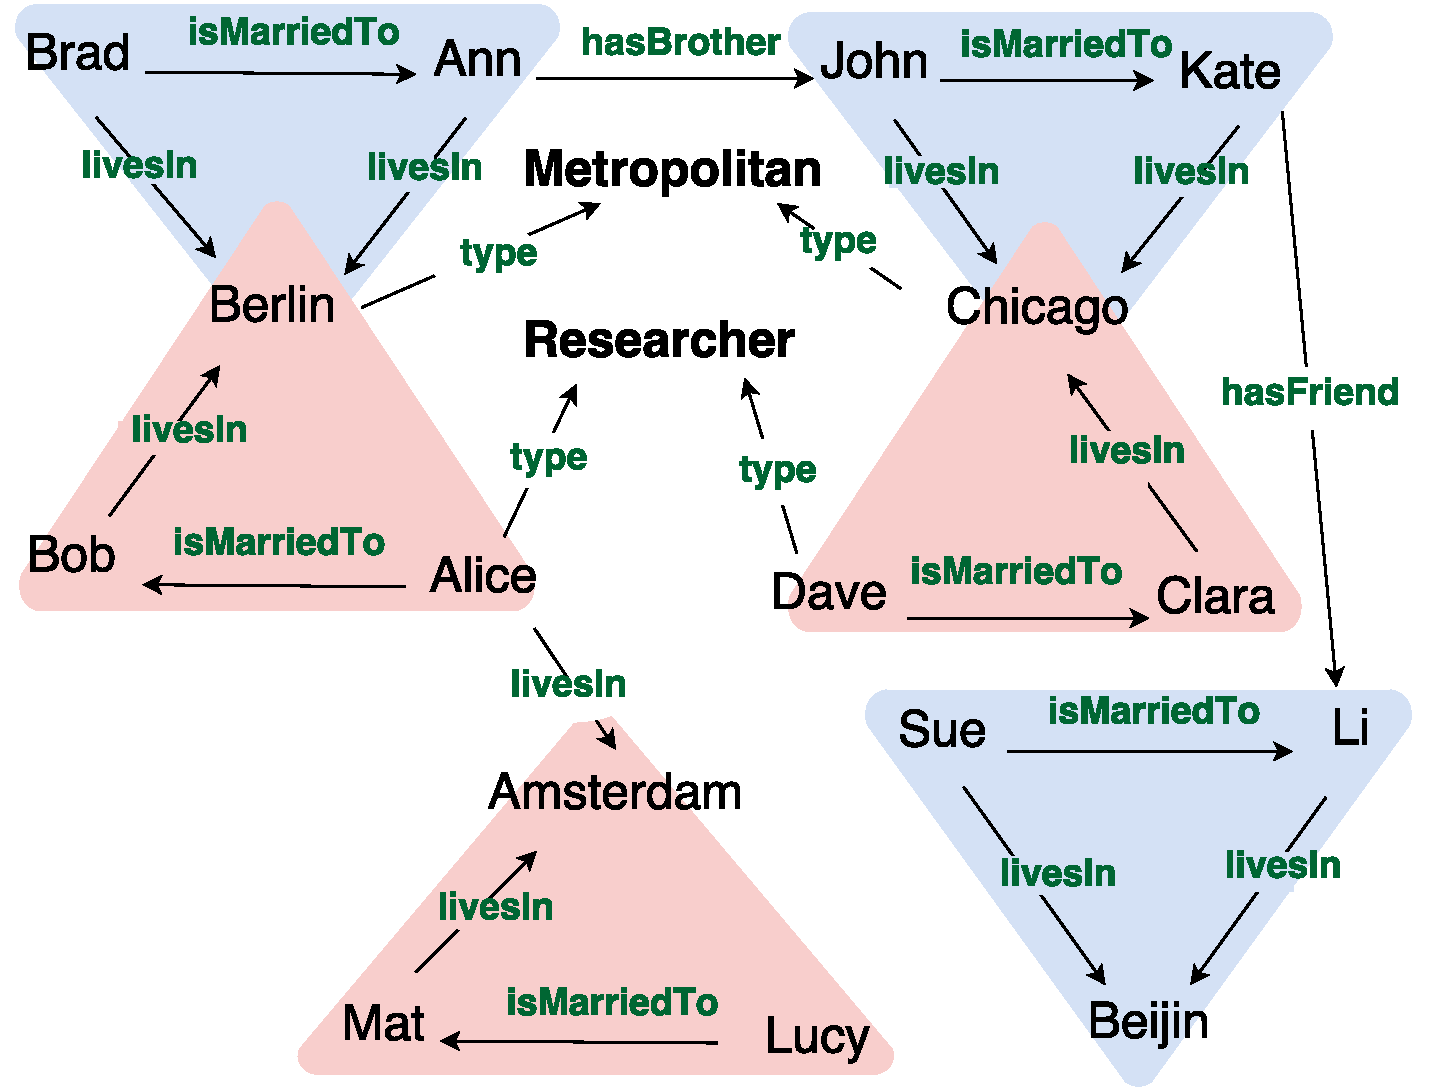
\includegraphics[width=0.57\textwidth]{figures/kg_advanced_col}
\caption{Example of a Knowledge Graph}
\label{rdf}
\end{figure}
Since KGs are automatically constructed, they are often \textit{incomplete}. %\ju{Suggestion: Replace the previous sentence with: "Since KGs are automatically constructed, they might contain mistakes and miss important information}. 
They are therefore naturally treated under the Open World Assumption (OWA). Also, the task of \textit{completion} (also known as \textit{link prediction}) is of crucial importance for the curation of KGs. To this aim, rule mining techniques (\textit{e.g.}, \cite{newrulemine,DBLP:journals/corr/WangL15i,amieplus}) have been exploited to automatically build rules able to make predictions on missing links. However, they mine Horn rules, which are insufficiently expressive to capture exceptions, and might therefore make incorrect predictions on missing facts.
% To complete and curate KGs, data mining techniques (\textit{e.g.}, \cite{newrulemine,DBLP:journals/corr/WangL15i,amieplus}) have been exploited to
% infer Horn rules. These, however, are insufficiently expressive to capture exceptions, and might therefore make incorrect predictions on missing facts.
For example, the following rule mined from the KG in Fig.~\ref{rdf} 
\begin{center}
$\mi{r1:\;livesIn(Z,Y)\leftarrow isMarriedTo(X,Z), livesIn(X,Y)}$ 
\end{center}
produces the following facts as conclusions: ${\mi{livesIn(alice{,}berlin)}}${,} ${\mi{livesIn(dave{,}chicago)}}$ and ${\mi{livesIn(lucy,amsterdam)}}$. However, the first two facts might be actually wrong link predictions.
%actually false; %\ju{ ("facts are actually false": this sounds weird in my ears. Why don't you simply say: "The application of rule r1 will predict two wrong facts: livesIn(alice, berlin), etc.)} DS: well, because due to the OWA we can not be sure about that
Indeed, both $\mi{alice}$ and $\mi{dave}$ are researchers, and the rule $\mi{r1}$ could be suspected to have $\mi{researcher}$ as a potential exception. In \cite{iswc2016}, a rule-based method for addressing this issue was proposed. It takes into account a cross-talk between the rules and aims at revising them to obtain a ruleset that describes the observed data well and predicts the unseen data consistently. However, it applies only to a flattened representation of a KG.
%\ju{ (what is a flattened representation? I liked more your commented version)}. DS: this is a standard term in ILP, which Francesca introduced here
%is limited to KGs with unary facts only. 

\section{Contributions}

In this paper we extend the results from \cite{iswc2016} to KGs in their original relational nature. %\ju{ (I'm not sure I understand what is a "relational nature" of the KG}.  
Basically, we reformulate the KG completion problem as a \textit{theory revision} problem, %\ju{(I would expand "problem" by stating more verbosly what is the problem that you tackle, i.e. the fact that mined association rules lead to wrong predictions}
where, given a KG and a set of (previously learned) Horn rules, the task is to compute a set of \textit{nonmonotonic rules} by adding default negated atoms to their bodies, such that the revised ruleset is more accurate than the original one.
We implemented %\ju{"implement"$\rightarrow$"implemented"} 
the developed extension and evaluated %\ju{"evaluate"$\rightarrow$"evaluated"} 
it on a real-world KG. 
Preliminary %\ju{"The"$\rightarrow$"(Our) preliminary"} 
experiments demonstrate the %\ju{the} 
effectiveness of our method and gains for the rule quality as well as the fact quality when performing KG completion. %\ju{I suggest you simplify this sentence with "Preliminary experiments indicate that our method is useful to improve the quality of the rules and hence to reduce the amount of wrong predictions (or something like this)"}.

%\comment{DS: why not traditional nonmonotonic rule learning algorithms}
%\comment{FL: I would postpone this discussion later in the paper}
% Our ultimate goal is to extract nonmonotonic logic programs from large KGs treated under OWA to reason about the available knowledge and add possibly missing facts to it. 
There are several important obstacles that prevent us from using the off-the-shelf ILP nonmonotonic rule learning algorithms:
\begin{itemize}
\item[1.] \textbf{Absence of target predicates for which the rules are to be learned.} In order to define target predicates for which we want to learn rules, we need to be aware of blank parts of our knowledge graph, i.e., predicates that are likely to be incomplete. For example, if we were aware that wikipedia contains very few data about playsInBand relation, we would focus only on this one and would exploit the existing ILP methods, but where would we get this knowledge from? There is a line of research that aims at determining parts of  a KG that are for sure complete, but how would we derive the knowledge about missing data? In the epistemic logic that would mean to learn what we do not know. Having this capability would open a wide range of possibilities; however, yet it is unclear where to get this data from.
% * <francesca.a.lisi@gmail.com> 2016-11-01T09:46:24.380Z:
%
% What is this relation? Where is it taken from?
%
% ^ <francesca.a.lisi@gmail.com> 2016-11-01T09:46:56.157Z.
\item[2.] \textbf{Absence of negative examples.} One might claim that a standard way of addressing (1) would be just try to learn relations for all predicates. This is obviously computationally expensive. Note that in our case, and in contrast to the standard formulation of the problem (see, \textit{e.g.}, \cite{wr1996}), the negative examples are not available due to the OWA. Thus the only possibility is to apply the positive only learning and extract rules for all of the relations in the given KG.
\item[3.] \textbf{Absence of language bias.} To restrict the search space of hypothesis one needs to set a concrete language bias. Since we do not know anything about the KG at hand, we have no idea about the form the potential rules should look like. To cope with this issue we first apply the association rule mining methods and then revise the rules accordingly by adding exceptions.
\end{itemize}
%\comment{FL: It is not appropriate to say that there is absence of the aforementioned ingredients. Better to say that they are difficult to obtain. I will rewrite this part.}
% Essentially, we are interested in tackling a \textit{theory revision} problem, in which as possible revision operations we are only allowed to add negated atoms to the antecedents of the rules. 
%, while the set of positive ones might be incomplete. 
%Thus, traditional methods cannot be applied. 
%\ju{(a citation of a "traditional method" would be useful here)}. DS: traditional method is cited above

% For example, triples of instances for which the rule $\mi{r1}$ does not hold are marked with colour in Figure~\ref{fig:rdf}.
% Hypothetical explanations why the rule does not hold, however, can only be found for the pairs $\mi{(bob, alice)}$ and $\mi{(clara,dave)}$.

Given the aforementioned difficulties, our method proceeds in four steps.
First, we compute what we call ``exception witnesses'': predicates that are
potentially involved in explaining exceptions (e.g., {\em researcher} in our example).
Second, we generate nonmonotonic rule candidates that we could possibly add to our KG rules.
Third, we devise quality measures for nonmonotonic rules to quantify their strength w.r.t the KG. In contrast to prior work, we do not merely give measures for individual rules in isolation,
but consider their cross-talk through a new technique that we call ``partial materialization''.
Fourth and last, we rank the nonmonotonic rules by their strengths and choose a cut-off point such that the obtained rules describe the KG's content as well as possible with awareness of exceptions.


The salient contributions of our paper are:
\begin{itemize}
\item A framework for nonmonotonic rule mining as a theory revision task,
to capture exceptions from Horn rules
and overcome the limitations of prior work on rule-based KG completion.
\item  An algorithm for computing exception candidates, measuring their quality,  and ranking them based on a novel technique
with \emph{partial materialization} of judiciously selected rules.
\item Experiments with the YAGO3 and IMDB KGs where we show the gains of our method for rule quality as well as fact quality when performing KG completion.
\end{itemize}

\section{Structure}

The paper is structured as follows. Sec.~\ref{sec:prelim} introduce preliminaries on nonmonotonic logic programming and relational association rule mining. Sec.~\ref{sec:rev_frame} describes our theory revision framework. Sec.~\ref{sec:meth} presents the methodology for computing an approximate solution whereas Sec.~\ref{sec:eval} reports experimental results. Sec.~\ref{sec:relwork} discusses the related work. Sec.~\ref{sec:concl} concludes the paper with final remarks and outlines directions of future work.

% \end{itemize}